\chapter{Introduction}
\label{cha:introduction}

% the code below specifies where the figures are stored
\ifpdf
    \graphicspath{{1_introduction/figures/PNG/}{1_introduction/figures/PDF/}{1_introduction/figures/}}
\else
    \graphicspath{{1_introduction/figures/EPS/}{1_introduction/figures/}}
\fi

\section{Motivation and Problem Statement}

A~very open definition of the word \emph{event}
given by WordNet~\cite{fellbaum1998wordnet,miller1995wordnet} is
\emph{``something that happens at a~given place and time''}.
Following this definition,
we are indeed surrounded by events,
most of little to no interest for us.
A~concert somewhere in the world of a~band
that we do not even know may be a~good example.
For some events, however, we may care more, for example,
a~concert of a~band that we know and like,
even if it takes place at a~location far away from us.
Finally, for very few events, we may care a~lot,
maybe even enough to physically attend the event,
like a~concert of our favorite band
if it takes place in our city, is not sold out,
and not too expensive.

All this motivates the need for \emph{event summarization}.
If there is an event that we could not attend
for a~reason whatsoever,
but that we are interested in,
a~good event summarization can help us get a~feeling
for the event's atmosphere.
Similarly, if there is an event that we attended,
we can revive the event's most fascinating moments
based on the event summarization.

A~\emph{media gallery} in the context of
our event summarization task is
a~compilation of photos, videos,
and microposts retrieved from social networks
that are related to a~given event.
Event summarization covers textual,
as well as multimedia content.
We say a~media gallery is of high quality,
if it fulfills the following properties.

\begin{enumerate}
  \item \textit{Conciseness:}
        they convey a~lot of information clearly
        and in few media items.
  \item \textit{Comprehensiveness:}
        they are complete, including all representative
        elements or aspects of an event.
  \item \textit{Authenticity:}
        they are of undisputed origin and genuine.
  \item \textit{Diversity:}
        they show a~great deal of variety.
  \item \textit{Interestingness:}
        they catch and hold the attention of the viewer.     
\end{enumerate}

\section{Research Question and Hypothesis}

The main research question for this thesis
can be formulated as follows.
 
\textit{``Can user-customizable
media galleries that summarize given events be
created solely based on textual and multimedia data
from social networks?''}

\noindent The hypothesis that we test in this thesis
can be formulated as follows.

We argue that
through media galleries that leverage content
shared on social networks
a~more \emph{authentic}, more \emph{concise},
more \emph{comprehensive}, more \emph{diverse},
and also more \emph{interesting}
view on events gets possible than by limiting oneself
to officially produced media content;
and that further such media galleries can be generated
more \emph{efficiently} and \emph{in shorter time}
than the officially produced ones.

We validate these subjective and objective
criteria with experiments for events of different categories
such as sports, politics, culture, leisure,
music, conferences, \emph{etc.}

\section{Approach}

The objective of this thesis is the development
of methods for the automatic summarization of events
based on media items shared on social networks.
A~schematic overview of the approach can be seen
in~\autoref{fig:thesis-diagram}.
As an event takes places and shortly thereafter
(symbolized by the timeline marked with \emph{2h Event}),
people share media items related to the event
on multiple social networks
(symbolized by the photo and video pictograms
above the event timeline).
Via the textual search functionality of those
different social networks,
we retrieve a~list of potentially event-relevant
microposts that either contain media items directly,
or that provide links to media items
on external media item hosting platforms.
Using third-party NLP tools,
we recognize and disambiguate named entities
in the microposts to predetermine their relevance.
We extract the binary media item data
from social networks or media item hosting platforms
and relate it to the originating microposts
(symbolized by the central cloud).
Using CBIR and CBVR techniques, we first deduplicate
exact and near-duplicate media items,
and then cluster similar media items
(symbolized by the green, red, and orange markers).
We rank the deduplicated and clustered list
of media items and their related microposts
according to well-defined ranking criteria.
In order to generate interactive and user-customizable
media galleries that visually and audibly summarize the
event in question, we compile the top-$n$ ranked
media items and microposts in an aesthetic way
(symbolized by the timeline marked with \emph{5min Summary}).

\begin{figure}[h!]
  \centering
  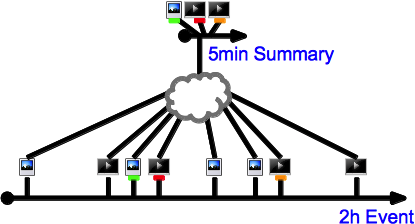
\includegraphics[]{thesis-diagram.png}
  \caption[Schematic depiction of event summary generation]
    {Schematic depiction of event summary generation
    based on deduplicated, clustered, and ranked media items
    for an exemplary event.}
  \label{fig:thesis-diagram}
\end{figure}

\section{Contributions}

In this thesis, we report on methods for
the automatic generation of event summaries.
This particular field of research touches on many related areas
of research and research communities,
amongst which social network research, multimedia content analysis,
Semantic Web and Natural Language Processing (NLP),
human factors in computing systems,
and Web services.
In consequence, we have broken our contributions down into
the following topics.

\subsection{Social Network Multimedia and Data Analysis}

We have worked on methods for the aggregation, extraction,
deduplication, clustering, and compilation
of social media contents from
multiple social networks.
\todo{What fresh media citation}
Those methods were applied and evaluated
for the enhancement of conference experiences.
\todo{Confomaton citations}

\subsection{Application of Semantic Web and NLP Techniques}

In order to make sense out of social network microposts,
we have worked on methods to consolidate and rank
the results of multiple named entity recognition and
disambiguation APIs and to track their data provenance.
\todo{Adding Meaning to Social Network citations}
We have applied and evaluated those methods
for the consumer-oriented detection of trending microposts
on a~major commercial social network.
\todo{A~tweet consumers' look citation}

\subsection{Video Content and Metadata Analysis}

We have worked on methods for named entity extraction and
disambiguation for online videos based on closed captions
and other textual metadata, which make online video
more accessible, searchable, and interconnected.
\todo{SemWebVid citation}
Further, we have combined those textual methods with 
video content analysis methods for the on-the-fly detection
of shot boundaries for online videos.
\todo{Enabling on-the-fly citation}
We have defined aesthetic principles
for the automatic generation of media gallery layouts
for visual and audial event summarization
based on social network multimedia data.
\todo{Defining aesthetic principles citation}
        
\subsection{Crowdsourcing}

The video content analysis methods mentioned before
were combined with methods for the crowdsourced detection
of events in online videos.
\todo{Crowdsourcing event detection citation}
We have further worked on crowdsourcing methods
for the extraction of knowledge items from arbitrary Web pages.
\todo{SEKI@home citations}

\subsection{Studies}

We have contributed an examination of Linked Data usage and
visualization techniques of a~major commercial search engine.
\todo{How Google is using citation}
In addition to that, we have studied the usefulness and relevance
of social network updates which were added to the search engine
results pages of a~major commercial search engine.
\todo{Adding real-time coverage citation}

\subsection{Multimodal Search Engines}

We have worked on an examination of context-aware querying
for multimodal search engines.
\todo{Context-aware querying citation}
Further, we have studied user interface constraints on
mobile and desktop devices for a~multimodal search engine
and demonstrated that those constraints can be overcome.
\todo{One size does not fit all citation}

\subsection{Web Services Description}

We have worked on methods for the semantic description of Web APIs,
their discoverability, their automatic consumption,
their semantic interlinking, and their social aspects.
\todo{RESTdesc citations}
We have studied the feasibility of truly RESTful behavior
for Web APIs in the sense of Dr. Roy Fielding.
\todo{Fulfilling the hypermedia constraint citation}
        
\subsection{Standardization and Specification}        
We have helped to shape a~W3C specification on media
fragment addressing schemes for audio and video items.
\todo{Media Fragments citation}
Further, we have worked on the definition of a~unified framework
for the description of multimedia content objects.
\todo{Introducing a~unified framework citation}
Finally, we have contributed to a~white paper on the
Future Media Internet Architecture.
\todo{FMIA citation}

\subsection{Others}

We have developed methods for unobtrusively fixing
common annoyances on arbitrary Web pages.
\todo{xkcd citation}

\section{Thesis Structure}

The remainder of this thesis is structured as follows. 
\todo{Add thesis structure}

Each chapter is closed by a~final section called
\emph{Chapter Notes}, which contains references to publications
that the chapter is based upon,
and in some cases pointers to related material for further reading.